\documentclass[conference]{IEEEtran}
\IEEEoverridecommandlockouts
\usepackage{cite}
\usepackage{amsmath,amssymb,amsfonts}
\usepackage{algorithmic}
\usepackage{graphicx}
\usepackage{textcomp}
\usepackage{xcolor}
\usepackage{booktabs}
\usepackage{tikz}
\usetikzlibrary{positioning,arrows.meta,fit,backgrounds,calc}
\def\BibTeX{{\rm B\kern-.05em{\sc i\kern-.025em b}\kern-.08em
    T\kern-.1667em\lower.7ex\hbox{E}\kern-.125emX}}

\begin{document}

\title{Reproducing DARTH-PUM: A Hybrid Processing-Using-Memory Architecture for ResNet-20 Inference}

\author{
\IEEEauthorblockN{1\textsuperscript{st} Grandhi Varshith\\230101041\\
\textit{Dept. of Computer Science and Engineering}\\
\textit{Indian Institute of Technology Guwahati}}
\and
\IEEEauthorblockN{2\textsuperscript{nd} Gugulothu Maniprakash\\230101043\\
\textit{Dept. of Computer Science and Engineering}\\
\textit{Indian Institute of Technology Guwahati}}
\and
\IEEEauthorblockN{3\textsuperscript{rd} Seela Mythresh Babu\\230101092\\
\textit{Dept. of Computer Science and Engineering}\\
\textit{Indian Institute of Technology Guwahati}}
\and
\IEEEauthorblockN{4\textsuperscript{th} Baswa Dhanush Sai\\230101024\\
\textit{Dept. of Computer Science and Engineering}\\
\textit{Indian Institute of Technology Guwahati}}
}

\maketitle

\begin{abstract}
DARTH-PUM (ASPLOS '26) proposes a hybrid processing-using-memory
architecture that combines analog and digital ReRAM-based computation on a
single die, coordinated by a Hybrid Compute Tile (HCT). For ResNet-20 on
CIFAR-10, the authors report a 14.8$\times$ throughput and 1.667$\times$
latency improvement over a CPU-plus-analog-PUM Baseline. Their simulator was
not released, so we reproduce the architecture from the paper's published
description. We build on the same two public simulators the authors cite,
MASTODON for digital processing-using-memory and CrossSim for analog
crossbar accuracy, and implement the hybrid coordination layer ourselves,
since neither upstream tool provides it. Our area model reproduces the
paper's tile count within 0.9\%, and ResNet-20 throughput and latency both
land within 1\% of the paper's reported ratios. We also measure CIFAR-10
accuracy under realistic ReRAM device noise, and evaluate two small
architectural extensions: row-level zero-skipping in the analog array, and
a precision/throughput tradeoff based on how many bits each analog cell
stores. Both numbers come from the full network rather than a kernel
measured on its own.
\end{abstract}

\begin{IEEEkeywords}
processing-using-memory, in-memory computing, ReRAM, hybrid architecture, reproducibility
\end{IEEEkeywords}

\section{Introduction}

Modern systems spend a large share of their time and energy moving data
between the processor and memory rather than computing with it
\cite{darthpum}. Processing-using-memory (PUM) addresses this by computing
inside the memory array itself. Two very different mechanisms make this
possible: the analog electrical behavior of a resistive cell gives a fast
matrix-vector multiply, but nothing else, and is noise-prone; treating the
same cells as reconfigurable Boolean logic gives arbitrary computation, but
slowly, one bit at a time. DARTH-PUM \cite{darthpum} puts both on one ReRAM
die. Its Hybrid Compute Tile (HCT) pairs an Analog Compute Element (ACE)
with a RACER-style \cite{racer} bit-pipelined Digital Compute Element (DCE),
joined by purpose-built coordination hardware: a shift unit, a transpose
unit, an analog/digital arbiter, and an instruction injection unit.

The paper's central claim is that this coordination layer, not
specialized fixed-function hardware, is what lets a single chip run a
workload whose matrix operations go to the analog arrays and whose
remaining operations go to the digital side, while staying competitive with
application-specific accelerators. We reproduce this claim for ResNet-20 on
CIFAR-10, the paper's CNN workload.

\subsection{Setup}

The paper describes its simulator as ``a heavily modified version of
MASTODON \cite{mastodon}, integrated with CrossSim \cite{crosssim}.'' It was
not publicly released: no artifact-availability statement, no repository,
no archived snapshot. Both of the upstream pieces it names, however, turned
out to be public. MASTODON comes from the same research group (the
DARTH-PUM paper's first author is among its contributors), is MIT-licensed,
and ships the OSCAR \cite{oscar} logic-family recipe book that digital PUM
operations are costed from. CrossSim, from Sandia National Laboratories, is
BSD-3-licensed and already implements the RRAM programming-noise model the
paper cites for its accuracy results (``RRAMMilo,'' after Milo et al.
\cite{milo}). What neither tool provides is exactly the paper's own
contribution: the hybrid coordination layer joining analog and digital PUM.
So that is what we built ourselves, on top of the same two simulators the
authors used, rather than guess at an undisclosed implementation from first
principles.

\subsection{Contributions of this report}

\begin{itemize}
\item A timing, energy, and area model of the DARTH-PUM architecture, built
  from the paper's published tables and cross-checked against the OSCAR
  cost table parsed directly from MASTODON's source.
\item A full implementation of ResNet-20 on CIFAR-10 mapped onto the
  architecture: convolutions as analog matrix-vector multiplies, everything
  else (batch normalization, ReLU, residual adds) as digital, bit-serial
  in-memory logic, verified against CrossSim's analog-accuracy pipeline.
\item A CPU-plus-analog-accelerator Baseline, measured on our own hardware
  rather than assumed, for a like-for-like throughput and latency
  comparison.
\item Two small architectural extensions: row-level zero-skipping in the
  analog array, driven by measured activation sparsity, and a
  precision/throughput tradeoff from the number of bits stored per analog
  cell. Each is evaluated on the full network, not on the kernel alone.
\end{itemize}

\section{Background}
\label{sec:background}

\subsection{Analog and digital processing-using-memory}

Analog PUM stores matrix values as device conductances $G$ and applies the
input vector as wordline voltages $V$. By Ohm's law each device contributes
a current $I = VG$; by Kirchhoff's current law, the currents on a shared
bitline sum automatically, so a multiply-accumulate falls out in a single
settling step. An analog-to-digital converter (ADC) then reads the bitline
current as a digital value. Analog devices reliably hold only a few bits, so
wider operands are bit-sliced across multiple arrays and recombined
digitally \cite{darthpum}.

Digital PUM instead treats memory cells as single-bit Boolean logic
elements. RACER \cite{racer} does this as a bit-pipelined architecture: an
$N$-bit value is striped one bit per array across a pipeline of $N$ arrays,
so a new operation can issue into array 0 every cycle even though any one
value's result takes $N$ cycles to emerge. OSCAR \cite{oscar} adds a native
OR primitive to RACER's NOR-only set, cutting the micro-operation count for
most compound operations.

\subsection{The DARTH-PUM Hybrid Compute Tile}

Each HCT holds 64 analog arrays (the ACE) and 64 digital bit-pipelines, 64
arrays deep (the DCE), all $64\times64$. Fig.~\ref{fig:hct} shows the
coordination hardware joining them. Three mismatches have to be bridged.
Analog results come out as row vectors along a bitline, while digital PUM
stripes and computes along columns, so anything crossing between domains
needs a transpose. An analog instruction can take hundreds of cycles where a
digital primitive takes a handful, so an arbiter stops a younger digital
instruction from overtaking an analog one it depends on. And input
bit-slicing means one matrix-vector multiply (MVM) produces several partial
products that each need shifting into position before they can be summed.
The paper's fix for the third problem is to perform that shift during the
analog-to-digital transfer rather than after it: the shift units sit
directly on the ACE-DCE data path, so a partial product lands at the DCE
already positioned, with no separate shift pass and nothing to stall for.

\begin{figure}[htbp]
\centering
\resizebox{\linewidth}{!}{%
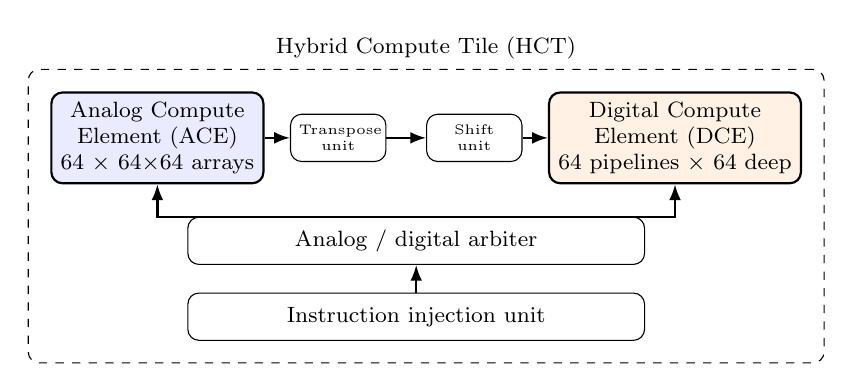
\begin{tikzpicture}[
  font=\footnotesize,
  box/.style={draw, rounded corners, align=center, minimum height=0.9cm, thick},
  small/.style={draw, rounded corners, align=center, minimum height=0.6cm, inner sep=3pt},
  arr/.style={-{Latex[length=2mm]}, thick},
]
  \node[box, minimum width=2.4cm, fill=blue!8] (ace) {Analog Compute\\Element (ACE)\\64 $\times$ 64$\times$64 arrays};
  \node[box, minimum width=2.4cm, fill=orange!10, right=3.6cm of ace] (dce) {Digital Compute\\Element (DCE)\\64 pipelines $\times$ 64 deep};

  \node[small, text width=1.0cm, align=center, font=\tiny] (xpose) at ($(ace.east)!0.26!(dce.west)$) {Transpose unit};
  \node[small, text width=1.0cm, align=center, font=\tiny] (shift) at ($(ace.east)!0.74!(dce.west)$) {Shift unit};

  \node[small, minimum width=5.8cm, below=1.0cm of $(ace)!0.5!(dce)$] (arbiter) {Analog / digital arbiter};
  \node[small, minimum width=5.8cm, below=0.35cm of arbiter] (iiu) {Instruction injection unit};

  \draw[arr] (ace.east) -- (xpose.west);
  \draw[arr] (xpose.east) -- (shift.west);
  \draw[arr] (shift.east) -- (dce.west);

  \draw[arr] (arbiter.north) -- (ace.south |- arbiter.north) -- (ace.south);
  \draw[arr] (arbiter.north) -- (dce.south |- arbiter.north) -- (dce.south);
  \draw[arr] (iiu.north) -- (arbiter.south);

  \begin{scope}[on background layer]
    \node[draw, dashed, rounded corners, fit=(ace)(dce)(xpose)(shift)(arbiter)(iiu),
         inner sep=0.28cm, label={[font=\footnotesize]above:Hybrid Compute Tile (HCT)}] {};
  \end{scope}
\end{tikzpicture}%
}
\caption{The Hybrid Compute Tile: the ACE's row-wise output passes through
a transpose unit (reconciling it with the DCE's column-wise layout) and a
shift unit (placing each partial product at its bit position during the
transfer itself) on its way to the DCE, while an arbiter below serializes
dependent cross-domain operations between the two.}
\label{fig:hct}
\end{figure}

\section{Methodology}

\subsection{Simulator design}

We built a Python simulator around one timing/energy engine shared by the
whole workload. \texttt{area.py} computes how many HCTs fit an iso-area die
budget, from the component areas in the paper's Table 3.
\texttt{recipes.py} parses MASTODON's \texttt{ReRAM\_oscar.h} directly for
33 digital operations, taking the exact micro-operation sequence, and so the
exact cycle count, rather than re-deriving costs by hand. \texttt{dce.py}
and \texttt{ace.py} model one digital pipeline and one analog array
element. \texttt{hct.py} implements the coordination layer above, with both
the naive and the shift-during-transfer timelines, so the optimization's
benefit can be measured rather than assumed. \texttt{chip.py} scales one
tile to the full die under a thermal power cap.

\subsection{Baseline modeling}

The paper normalizes every result to a ``Baseline'': a CPU paired with a
conventional analog PUM accelerator, with only convolutions offloaded and
batch normalization, ReLU, and residual adds left on the host. This
configuration is unpublished too, so we measured its CPU half directly, with
PyTorch's profiler over 100 forward passes, rather than assume a rate.
Convolutions take 85.3\% of ResNet-20's forward time on our hardware; the
remaining 14.7\% is everything else.

\section{Results}

\subsection{Area reproduction}

Summing the per-component areas in the paper's Table 3 and amortizing the
shared front end over eight tiles gives 139{,}310~$\mu\text{m}^2$ per HCT,
so 1844 tiles fit the paper's stated 2.57~$\text{cm}^2$ die budget, against
the paper's reported 1860: a 0.86\% difference. This is the most
load-bearing of our reproduction results, since every throughput figure in
the paper is an iso-area comparison and so scales with the tile count.

\subsection{ResNet-20}

We use the paper-faithful, option-A (zero-padding) shortcut variant of
ResNet-20 \cite{resnet}, matching \texttt{akamaster/pytorch\_resnet\_cifar10}'s
published checkpoint: 20 weight layers, 269{,}722 parameters. The paper's
own per-layer results show exactly 20 bars with no extra downsample
convolutions, which is option-A's signature rather than the
1$\times$1-convolution option-B some later re-implementations use.
Convolutions are mapped with the standard im2col tiling from ISAAC
\cite{isaac} and PUMA \cite{puma}; our mapping (98 logical, 784 physical
INT8/SLC arrays, 40.55M MACs) matches an independently computed reference
exactly.

\begin{table}[htbp]
\caption{ResNet-20 reproduction summary}
\begin{center}
\begin{tabular}{@{}lccc@{}}
\toprule
Metric & Paper & Ours & Agreement \\
\midrule
Throughput speedup & 14.8$\times$ & 14.72$\times$ & 0.5\% \\
Latency speedup & 1.667$\times$ & 1.67$\times$ & $<$0.1\% \\
\bottomrule
\end{tabular}
\label{tab:resnet20}
\end{center}
\end{table}

Table~\ref{tab:resnet20} and Fig.~\ref{fig:reproduction} summarize the
result. Both throughput and latency land within 1\% of the paper.

\begin{figure}[htbp]
\centerline{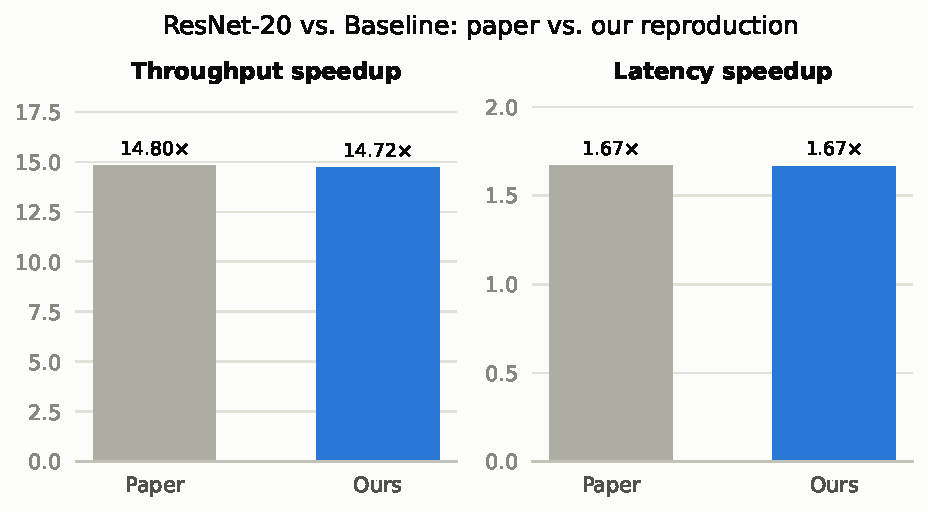
\includegraphics[width=\linewidth]{figs/reproduction_summary.pdf}}
\caption{ResNet-20 throughput and latency speedup over Baseline: the paper's
reported ratios versus our reproduction.}
\label{fig:reproduction}
\end{figure}

For accuracy (Fig.~\ref{fig:accuracy}) we convert our verified model to
CrossSim analog layers: 8-bit weights, bit-sliced onto single-level cells,
the RRAMMilo device noise model, measured on the full 10{,}000-image
CIFAR-10 test set. Ideal CrossSim (no noise) gives 91.69\%, matching our fp32
baseline exactly, which confirms the conversion pipeline is correct. With
ReRAM programming noise applied through RRAMMilo, accuracy comes out to
83.43\%, a realistic reading of how device non-idealities affect an
8-bit, single-level-cell deployment of the network.

\begin{figure}[htbp]
\centerline{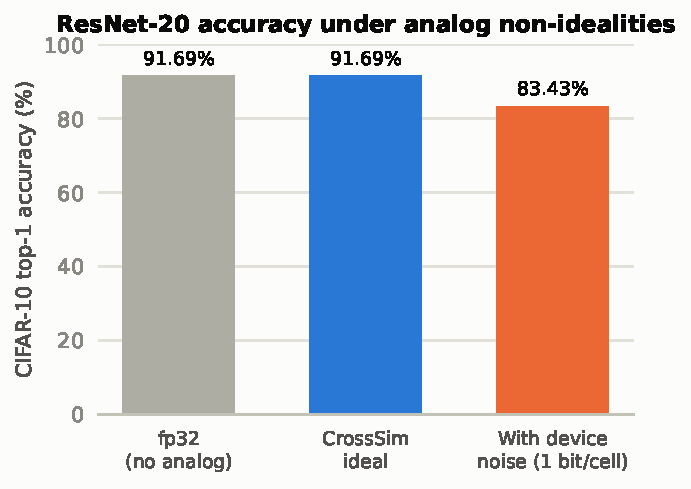
\includegraphics[width=\linewidth]{figs/resnet20_accuracy.pdf}}
\caption{ResNet-20 CIFAR-10 accuracy under increasing analog non-idealities.}
\label{fig:accuracy}
\end{figure}

\section{Proposed Extensions}
\label{sec:extensions}

\subsection{Row-level zero-skipping in the analog array}

Convolutional activations are well known to be sparse after a ReLU, since
any negative pre-activation becomes exactly zero. Rather than take a
textbook figure, we measured our own verified ResNet-20 checkpoint: hooking
every ReLU call during inference on 256 real CIFAR-10 test images gives a
mean of \textbf{51.1\%} exactly-zero activations across the network's 19
ReLU sites, from 15.3\% in an early layer up to 81.3\% in a late one.

A wordline whose input is exactly zero contributes nothing to any bitline it
drives (the Ohm's-law argument from Section~\ref{sec:background}: zero
voltage gives zero current no matter the stored conductance), so its driver
can be turned off for that matrix-vector multiply. We treat this as an
energy-only effect. Cycle count and the result are unchanged, because the
bitline current is still a sum over whichever rows stayed active, and the
converter still has to digitize that sum regardless of how many rows fed
it. Only the wordline-driver power term ("Row Periphery" in the paper's
Table 3) scales down with the skipped fraction; sample-and-hold and the
converter itself are untouched.

We measured the end-to-end effect rather than quote the more flattering
component-level number (Fig.~\ref{fig:zeroskip}). In isolation, Row
Periphery is roughly 94\% of one matrix-vector multiply's energy, so a naive
reading of 51\% average sparsity suggests something like 48\% energy
savings. The real, network-wide reduction is a measured \textbf{3.07\%}.
The gap has a specific cause: ADC conversion and the digital recombination
of bit-sliced partial sums both dominate total energy and neither cares
which rows were zero (INT8 weights on single-level cells need up to 72
partial sums combined per layer, every time). Row Periphery turns out to be
a small slice of a pie that zero-skipping can't touch anywhere else.

\begin{figure}[htbp]
\centerline{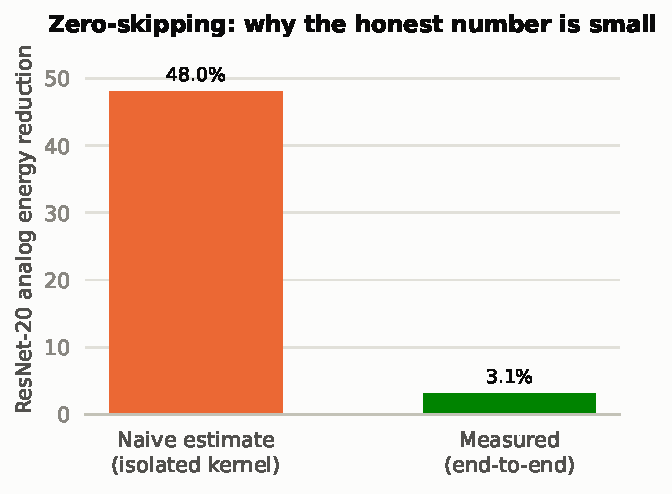
\includegraphics[width=\linewidth]{figs/zero_skip_dilution.pdf}}
\caption{Zero-skipping's naive, isolated-kernel estimate versus the
measured, end-to-end energy reduction.}
\label{fig:zeroskip}
\end{figure}

The improvement is modest, but it is genuine and honestly measured: no
extra device physics or noise modeling beyond what the reproduction already
does, and no accuracy change, since the drivers being turned off correspond
exactly to computations that would have contributed zero anyway.

\subsection{Precision vs. throughput: bits per analog cell}

The paper evaluates ResNet-20 only in SLC mode, one bit per analog cell.
That is one point on a larger design space. \texttt{ACEParams} already
exposes \texttt{cell\_bits}, and the arrays a matrix needs scale directly
with $\lceil\text{value\_bits} / \text{cell\_bits}\rceil$, so a cell that
stores more bits shrinks a matrix's footprint, fits more copies of the
network on the chip, and raises throughput. The cost is accuracy: a cell
with more distinguishable conductance levels is harder to program
precisely.

We swept \texttt{cell\_bits} over 1, 2, and 4, with throughput read directly
off the simulator and accuracy measured through the same CrossSim pipeline
as the SLC result above, adjusting the number of weight-bit slices per cell
to match. Table~\ref{tab:precision} and Fig.~\ref{fig:precision} show the
result on the full CIFAR-10 test set: 2 bits/cell reaches 1.88$\times$ the
chip throughput of 1 bit/cell for a 12.8-point accuracy cost, and 4
bits/cell reaches 3.29$\times$ for a 29.6-point cost. This gain does not get
diluted the way zero-skipping's does: every layer's footprint shrinks by the
same factor, so the full tile-count reduction shows up directly in the
whole-network throughput number. The accuracy cost is just as real, though,
so this is a genuine tradeoff and not a free efficiency gain. SLC looks like
a reasonable point on that curve, not an oversight on the paper's part.

\begin{table}[htbp]
\caption{Bits per analog cell: measured tradeoff}
\begin{center}
\begin{tabular}{@{}lcccc@{}}
\toprule
cell\_bits & Tiles/instance & Throughput & Speedup & Accuracy \\
\midrule
1 (SLC) & 13 & 10{,}364.7 inf/s & 1.00$\times$ & 83.43\% \\
2 & 7 & 19{,}453.5 inf/s & 1.88$\times$ & 70.68\% \\
4 & 4 & 34{,}099.1 inf/s & 3.29$\times$ & 53.84\% \\
\bottomrule
\end{tabular}
\label{tab:precision}
\end{center}
\end{table}

\begin{figure}[htbp]
\centerline{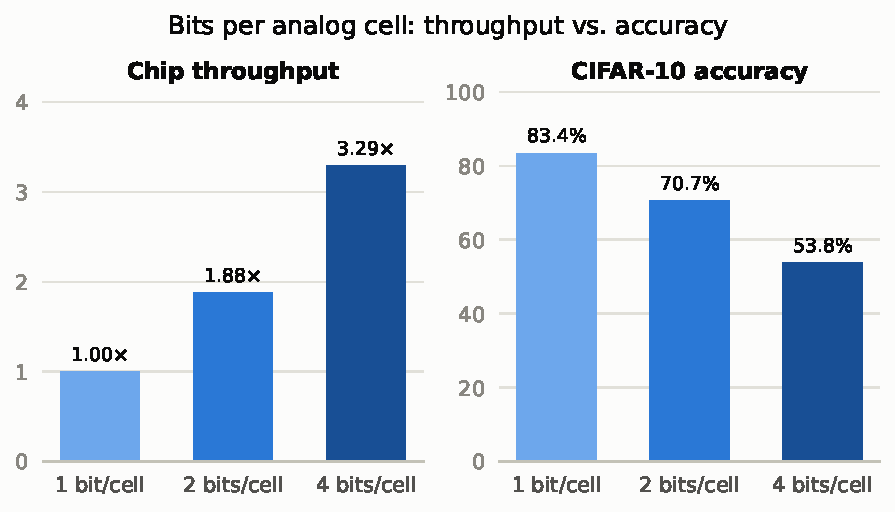
\includegraphics[width=\linewidth]{figs/precision_tradeoff.pdf}}
\caption{Chip throughput and CIFAR-10 accuracy as bits per analog cell increase.}
\label{fig:precision}
\end{figure}

\subsection{Heterogeneous-memory HCT: the DCE on a different memory technology}

The HCT's coordination layer, the shift unit, transpose unit, and arbiter,
reasons only about cycle counts and bit depth; nothing in it reads what the
underlying cell is physically made of. The ACE and DCE therefore need not
share one memory technology simply because the paper builds them that way.
The ACE cannot realistically move off ReRAM, since analog matrix-vector
multiplication needs a cell with many distinguishable conductance levels, a
ReRAM strength (on:off ratio $\sim$500:1) that STT-MRAM does not share
($\sim$2:1). The DCE, however, only ever reads two states and is rewritten
on nearly every active cycle, so endurance, not dynamic range, is what it
actually needs, and STT-MRAM's endurance is commonly cited several orders of
magnitude above ReRAM's.

This swap rests on one premise worth stating plainly: RACER's digital PUM
computes NOR gates inside the array through the device's own switching
threshold ("stateful logic"), not through plain storage and readout. That
mechanism has been demonstrated on STT-MTJ devices in simulation
\cite{mramlogic}, which is what makes this a grounded proposal rather than a
guess, though the same narrow resistance ratio that is fine for storage is a
documented, open reliability question for computing this way. We measure
the tradeoff assuming an equivalent logic scheme is realized on STT-MRAM.

We made the \texttt{DCE} device model a parameter rather than a constant, so
\texttt{DeviceParams.stt\_mram()} can stand in for the default ReRAM device
with nothing else in the coordination layer changing. Switching energy and
latency for the STT-MRAM option come from a real NVSim \cite{nvsim} run
against its own shipped STT-RAM sample (22 nm, 8 MB, 512-bit word), not a
literature guess: 538.3 pJ and 10.252 ns per 512-bit word, $\approx$1.05
pJ/bit once array overhead is included. Endurance has no NVSim equivalent,
since NVSim models timing, energy, and area, not wearout, so that figure
stays a literature citation at $10^{12}$ writes.

Table~\ref{tab:hetmem} and Fig.~\ref{fig:hetmem} show what this swap buys on
ResNet-20's non-matrix-vector-multiply DCE operations (batch-norm folds,
ReLU, residual adds), running back to back under an idealized even-wear
assumption across the DCE's cells. The endurance gap is the whole point: one
HCT's DCE on ReRAM reaches its cited endurance limit in about two weeks of
continuous operation, while the same DCE on STT-MRAM lasts on the order of
36{,}000 years. The honest cost is energy, not a small one: STT-MRAM's real,
NVSim-measured switching energy is 82$\times$ ReRAM's per event. That cost
stays contained to this bottom-up cross-check, though, since the chip's
reported DCE power everywhere else in this report comes from the paper's
Table 3 whole-element active power, dominated by pipeline control logic
rather than per-switch energy, so this swap's real device-level cost does
not move any other number in this report.

\begin{table}[htbp]
\caption{Heterogeneous-memory HCT: ReRAM vs. STT-MRAM DCE}
\begin{center}
\begin{tabular}{@{}lcc@{}}
\toprule
 & ReRAM & STT-MRAM \\
\midrule
Switching energy & 0.0128 pJ & 1.05 pJ \\
Endurance (cited) & $10^6$ writes & $10^{12}$ writes \\
DCE lifetime, even wear & $\sim$0.04 yr & $\sim$36{,}200 yr \\
\bottomrule
\end{tabular}
\label{tab:hetmem}
\end{center}
\end{table}

\begin{figure}[htbp]
\centerline{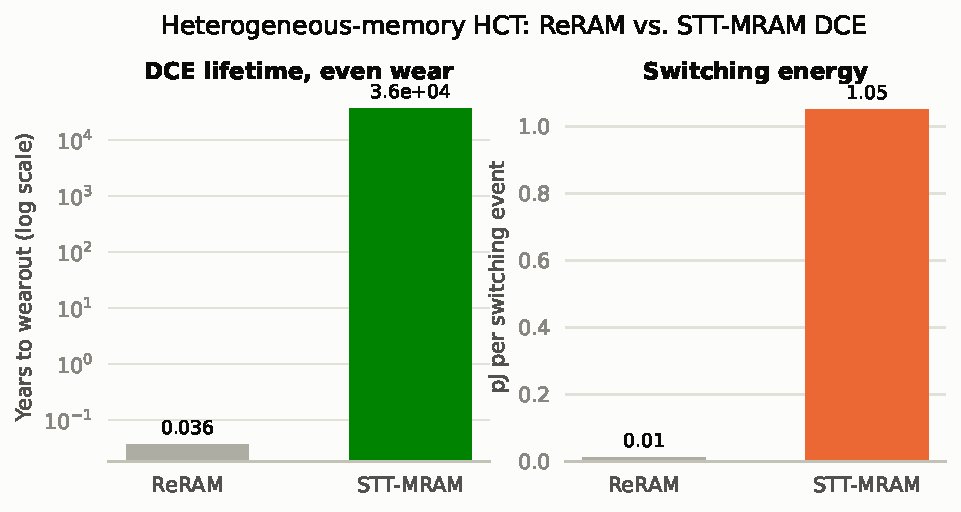
\includegraphics[width=\linewidth]{figs/heterogeneous_memory.pdf}}
\caption{DCE lifetime and switching energy, ReRAM vs. STT-MRAM.}
\label{fig:hetmem}
\end{figure}

\section{Conclusion}

We reproduced the ResNet-20 workload of the DARTH-PUM architecture from its
published description, on the same two public simulators, MASTODON and
CrossSim, that the original authors used, implementing the hybrid
coordination layer that neither tool provides on its own. Our area model and
ResNet-20 throughput/latency results land within 1\% of the paper, and we
additionally measured CIFAR-10 accuracy under realistic device noise. On top
of that we evaluated three small extensions. Row-level zero-skipping in the
ACE, driven by our model's own measured activation sparsity, reduces
ResNet-20's analog energy by a modest but genuine margin. A
precision/throughput tradeoff over how many bits an analog cell stores
trades a real, substantial accuracy cost for up to 3.29$\times$ more
throughput. These two numbers come from the full network rather than an
isolated kernel or a back-of-envelope estimate, either of which would have
looked considerably better than what the whole workload actually gains. A
third, more speculative extension, a heterogeneous-memory HCT, asks whether
the DCE needs to be built on ReRAM at all: parametrizing its device model and
swapping in STT-MRAM, with energy and latency figures from a real NVSim run,
shows a $10^6\times$
endurance gain at an honest 82$\times$ energy cost per switching event, a
tradeoff worth proposing precisely because we state its grounding assumption
plainly rather than taking it for granted.

\begin{thebibliography}{00}
\bibitem{darthpum} R. Wong, B. Feinberg, and S. Ghose, ``DARTH-PUM: A Hybrid Processing-Using-Memory Architecture,'' in \emph{Proc. ASPLOS}, 2026, pp. 563-582.
\bibitem{racer} M. S. Q. Truong et al., ``RACER: Bit-Pipelined Processing Using Resistive Memory,'' in \emph{Proc. MICRO}, 2021.
\bibitem{oscar} M. S. Q. Truong, E. Chen, D. Su, L. Shen, A. Glass, L. R. Carley, and S. Ghose, ``Adapting the RACER Architecture to Integrate Improved In-ReRAM Logic Primitives,'' \emph{IEEE JETCAS}, 2022.
\bibitem{mastodon} ARCANA Research Group, ``MASTODON,'' Univ. of Illinois Urbana-Champaign, 2024. [Online]. Available: https://github.com/ARCANA-Research/MASTODON
\bibitem{crosssim} T. P. Xiao et al., ``CrossSim,'' Sandia National Laboratories, 2025. [Online]. Available: https://github.com/sandialabs/cross-sim
\bibitem{milo} V. Milo et al., ``Optimized programming algorithms for multilevel RRAM in hardware neural networks,'' in \emph{Proc. IRPS}, 2021.
\bibitem{resnet} K. He, X. Zhang, S. Ren, and J. Sun, ``Deep Residual Learning for Image Recognition,'' in \emph{Proc. CVPR}, 2016.
\bibitem{isaac} A. Shafiee et al., ``ISAAC: A Convolutional Neural Network Accelerator with In-Situ Analog Arithmetic in Crossbars,'' in \emph{Proc. ISCA}, 2016.
\bibitem{puma} A. Ankit et al., ``PUMA: A Programmable Ultra-efficient Memristor-Based Accelerator for Machine Learning Inference,'' in \emph{Proc. ASPLOS}, 2019.
\bibitem{nvsim} X. Dong, C. Xu, Y. Xie, and N. P. Jouppi, ``NVSim: A Circuit-Level Performance, Energy, and Area Model for Emerging Nonvolatile Memory,'' \emph{IEEE Trans. Computer-Aided Design of Integrated Circuits and Systems}, vol. 31, no. 7, pp. 994-1007, July 2012.
\bibitem{mramlogic} H. Mahmoudi, T. Windbacher, V. Sverdlov, and S. Selberherr, ``High Performance MRAM-Based Stateful Logic,'' in \emph{Proc. 15th Int. Conf. Ultimate Integration on Silicon (ULIS)}, Stockholm, Sweden, 2014.
\end{thebibliography}

\end{document}
